\section{Problem 1 - Analytical}
\textit{Derive the expressions for the reflection and transmission coefficients for vertically polarized incident waves.}\\

This derivation is done in analogy to the one given in the lecture for horizontally polarized incident waves (see \figref{fig:mm12_1_H}). For vertically polarized incident waves, the setting at the boundary is shown in \figref{fig:mm12_1_V}. Considering the boundary conditions for the electric and magnetic fields, two equations which can be found which give the conditions to avoid discontinuities at the boundary. 

 \begin{figure} [!h]
 \centering
 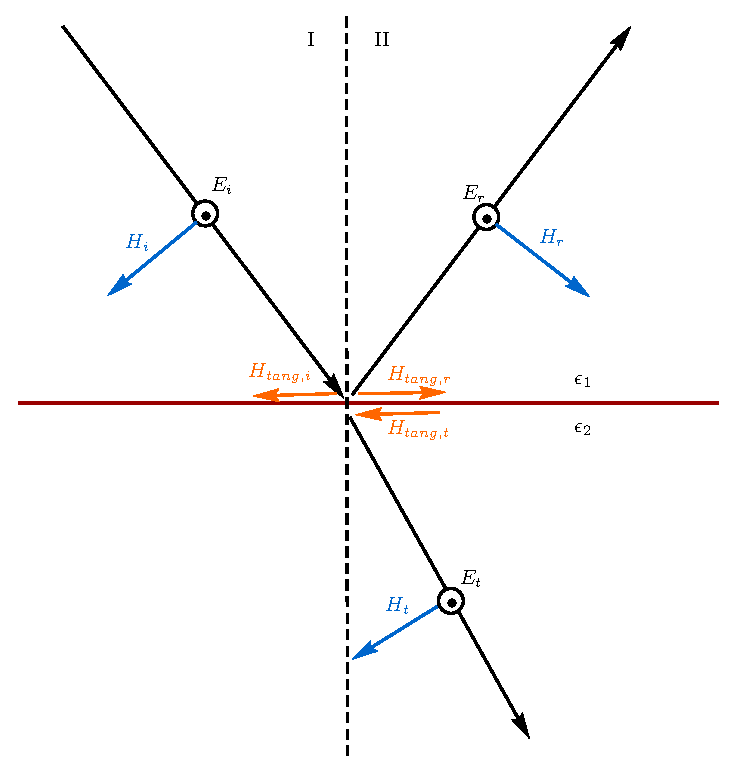
\includegraphics[width=8cm]{figures/mm12_1_H.eps}
 \caption{Setting for horizontally polarized incident waves.} \label{fig:mm12_1_H}
 \end{figure}

 \begin{figure} [!h]
 \centering
 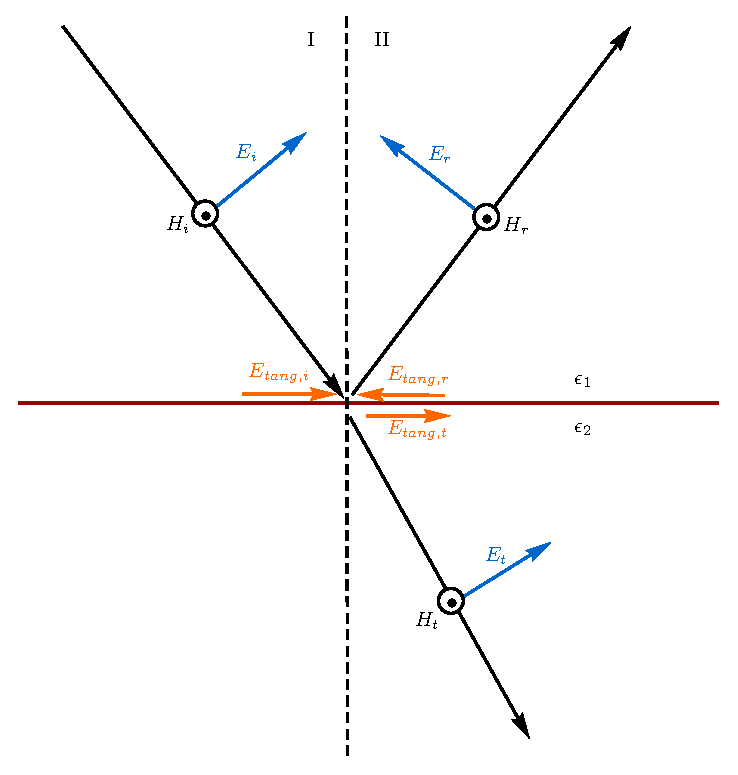
\includegraphics[width=8cm]{figures/mm12_1_V.eps}
 \caption{Setting for vertically polarized incident waves.} \label{fig:mm12_1_V}
 \end{figure}

\begin{flalign}
&& H_i &= H_t+H_r & \label{eq:E_all_ii} &\\
&& E_{i\lvert \rvert} &= E_{t\lvert \rvert} - E_{r\lvert \rvert} & \label{eq:E_all_i}
\end{flalign}

The parallel electric field components from \eqref{eq:E_all_i} are calculated by the actual field and the cosine of the angle yielding

\begin{flalign}
E_i e^{-j k_1 \sin(\theta_i)x} \cos(\theta_i) = E_t e^{-j k_2 \sin(\theta_t)x} \cos(\theta_t) - E_r e^{-j k_1 \sin(\theta_r)x} \cos(\theta_r) \label{eq:E_Tv}
\end{flalign}

which can be simplified knowing that $\theta_i=\theta_r$. The minus-sign is important and can be found comparing the directions of the field components shown in \figref{fig:mm12_1_V}. Sorting this equation for $E_t$, we get

\begin{flalign}
E_t  = \frac{ E_i e^{-j k_1 \sin(\theta_i)x} \cos(\theta_i) + E_r e^{-j k_1 \sin(\theta_i)x}  \cos(\theta_i)}{e^{-j k_2 \sin(\theta_t)x}  \cos(\theta_t)} \label{eq:E_t_i}
\end{flalign}

The second equation for $E_t$ can be found from \eqref{eq:E_all_ii}. The electric and magnetic field are coupled by the wave impedances of the individual materials $\eta$. These are dependant on the respective $\epsilon$.

\begin{flalign}
\frac{E_i}{\eta_1} e^{-j k_1 \sin(\theta_i)x}  =\frac{E_t}{\eta_2} e^{-j k_2 \sin(\theta_t)x}   + \frac{E_r}{\eta_1} e^{-j k_1 \sin(\theta_r)x}  
\end{flalign}

which results in 

\begin{flalign}
E_t  = \eta_2 \frac{\frac{E_i}{\eta_1} e^{-j k_1 \sin(\theta_i)x}  - \frac{E_r}{\eta_1} e^{-j k_1 \sin(\theta_i)x} }{ e^{-j k_2 \sin(\theta_t)x} } 
\end{flalign}

for $E_t$. With \eqref{eq:E_t_i} the relationship between $E_r$ and $E_i$ is then given as 

\begin{flalign}
&& \frac{\left( E_i   + E_r  \right) e^{-j k_1 \sin(\theta_i)x} \cos(\theta_i)}{e^{-j k_2 \sin(\theta_t)x}  \cos(\theta_t)} &= \eta_2 \frac{\left( \frac{E_i}{\eta_1}   - \frac{E_r}{\eta_1} \right) e^{-j k_1 \sin(\theta_i)x} }{ e^{-j k_2 \sin(\theta_t)x} }  &\\
&& \left( E_i   + E_r  \right) \frac{ \cos(\theta_i)}{ \cos(\theta_t)} &= \eta_2 \left( \frac{E_i}{\eta_1}   - \frac{E_r}{\eta_1} \right)  & \\
&& E_r \left( \frac{\cos(\theta_i)}{\cos(\theta_t)}  + \frac{\eta_2}{\eta_1} \right)  &= E_i \left( -\frac{\cos(\theta_i)}{\cos(\theta_t) } + \frac{\eta_2}{\eta_1}  \right) &\\
&& \frac{E_r}{E_i}  &= \frac{ -\frac{\cos(\theta_i)}{\cos(\theta_t) } + \frac{\eta_2}{\eta_1}  }{ \frac{\cos(\theta_i)}{\cos(\theta_t)}  + \frac{\eta_2}{\eta_1} } &\\
&& &=\frac{  \frac{\eta_2}{\eta_1} \cos(\theta_t)  -\cos(\theta_i)}{\frac{\eta_2}{\eta_1} \cos(\theta_t)  + \cos(\theta_i)}  &
\end{flalign}

The ratio between $E_r$ and $E_i$ is the reflection coefficient $R_v$ we are looking for. The ratio of the wave impedances can be transformed into a ratio of permittivities:

\begin{flalign}
\frac{\eta_2}{\eta_1} = \sqrt{ \frac{\epsilon_1}{\epsilon_2}}
\end{flalign}

Also, $\cos(\theta_t)$ can be expressed in terms of $\theta_i$ using Snells Law.

\begin{flalign}
&& \cos(\theta_t) &= \sqrt{ 1 - \sin^2(\theta_t) }&\\
&& &= \sqrt{ 1 - \frac{\epsilon_1}{\epsilon_2}\sin^2(\theta_i) } &
\end{flalign}

Now the given formula for the reflection coefficient can be derived.

\begin{flalign}
&& R_v &=\frac{  \sqrt{ \frac{\epsilon_1}{\epsilon_2}} \sqrt{ 1 - \frac{\epsilon_1}{\epsilon_2}\sin^2(\theta_i) }  -\cos(\theta_i)}{\sqrt{ \frac{\epsilon_1}{\epsilon_2}} \sqrt{ 1 - \frac{\epsilon_1}{\epsilon_2}\sin^2(\theta_i) }  + \cos(\theta_i)}  &\\
&& &=   \frac{ \sqrt{ \frac{\epsilon_1}{\epsilon_2} - \left( \frac{\epsilon_1}{\epsilon_2} \right)^2 \sin^2(\theta_i) }  -\cos(\theta_i)}{\sqrt{ \frac{\epsilon_1}{\epsilon_2} - \left( \frac{\epsilon_1}{\epsilon_2} \right)^2 \sin^2(\theta_i) }  + \cos(\theta_i)}     &\\
&& &=   \frac{ \sqrt{ \frac{\epsilon_2}{\epsilon_1}  -  \sin^2(\theta_i) }  - \frac{\epsilon_2}{\epsilon_1} \cos(\theta_i)}{\sqrt{ \frac{\epsilon_2}{\epsilon_1}  -  \sin^2(\theta_i) }  + \frac{\epsilon_2}{\epsilon_1} \cos(\theta_i)} &\\ 
&& &= \frac{ \frac{\epsilon_2}{\epsilon_1} \cos(\theta_i) - \sqrt{ \frac{\epsilon_2}{\epsilon_1}  -  \sin^2(\theta_i) }  }{\frac{\epsilon_2}{\epsilon_1} \cos(\theta_i) + \sqrt{ \frac{\epsilon_2}{\epsilon_1}  -  \sin^2(\theta_i) }} &
\end{flalign}

The transmission coefficient $T_v=\frac{E_t}{E_i}$ can be calculated using $R_v$ and \eqref{eq:E_Tv}. In addition to that, the relation $\sin(\theta_t)=\frac{k_1}{k_2} \sin(\theta_r)$ yields that 

\begin{flalign}
&& e^{-j k_2 \sin(\theta_t) x} &= e^{-j k_2 \frac{k_1}{k_2} \sin(\theta_r)x}  &\\
&& &= e^{-j k_1 \sin(\theta_i)x}
\end{flalign}

which simplifies \eqref{eq:E_Tv} to

\begin{flalign}
&& E_i  &= E_t \cos(\theta_t) - E_r \cos(\theta_i) &\\
&& \frac{E_i}{E_i} &= \frac{E_t}{E_i} \cos(\theta_t) - \frac{E_r}{E_i}\cos(\theta_i) &\\
&& 1 &= T_v \cos(\theta_t) - R_v \cos(\theta_i) &\\
&& (1-R_v) \cos(\theta_t) &= T_v \cos(\theta_i) &\\
&& T_v &= (1-R_v) \frac{\cos(\theta_i)}{\cos(\theta_t)} &
\end{flalign}